\documentclass[25pt, a0paper,
               colspace=15mm, subcolspace=0mm,
               blockverticalspace=17mm, margin=1in, total={35in, 44in},
               landscape]{tikzposter} % See Section 

\usepackage{poster}
\usepackage{array}
\usepackage{multirow}
\usepackage{multicol}
%\usepackage[table,xcdraw]{xcolor}

\definecolor{PaleBlue}{rgb}{0,.55,.9}
\definecolor{PaleGreen}{rgb}{0,.7,.25}
\definecolor{RedPink}{rgb}{.9,0,.2}
\definecolor{Pink}{rgb}{.85,.35,.7}
\definecolor{Purple}{rgb}{.6,0,.75}
\definecolor{Orange}{rgb}{.9,.3,.05}

\colorlet{attentionColor}{Orange}
\colorlet{charEmbedColor}{RedPink}
\colorlet{predEmbedColor}{Pink}
% \colorlet{attentionColor}{GoldUL!90!black}
% \definecolor{attentionColor}{rgb}{.85,.5,.6}



\def\pathwidth{2pt}
\def\nodewidth{3pt}
\def\cornerCurvature{7pt}

\tikzstyle{embed}=[%
  draw,
  #1,
  % line width=3pt,
  anchor=north,
  minimum width=.8cm,
  minimum height=1.6cm,
  inner sep=0pt,
  text=#1!65!black,
  font=\fontsize{25pt}{24}\selectfont,
  ]

\title{\parbox{\linewidth}{\centering Applying Pruning Filters In Convolutional Neural Network}}
\institute{Department of Computer Science and Software Engineering, Université Laval}
\author{Vincent Martineau}

\begin{document}
\maketitle

\begin{columns}
\column{.4}
\block{Introduction}{%
It was shown in P.Molchanov et al. that it was possible to prune a convolution neural network and still have decent results. However the proposed solution might require a lot of iterations. In the case we need more complex model to run on smaller device(Jetson) and prototype quickly there are some properties that seems consistent and that could improve workflow.

\vspace{15mm}
\textbf{Related work:}
\begin{itemize}
  \item P.Molchanov et al. (2017): Pruning Convolutional Neural Networks for Resource Efficient Inference.
  \item H.Li et al. (2017): Pruning Filters for Efficient ConvNets.
\end{itemize}

\vspace{0mm}
\textbf{Goals:}
\begin{itemize}
  \item Reduce training time to produce sufficient network.
  \item Provide a module that could handle multiple models.
   \item Explore the effect of pruning for speed and size.
\end{itemize}
}

\column{0.30}
\block{Algorithm}{
\begin{itemize}
	\item Do initial training (not complete)
	\item \textbf{Prepare Pruning}
	\begin{itemize}
		\item Convert model to ONNX
		\item Extract execution graph and Determine which layer can be pruned
	\end{itemize}
	\item \textbf{Prune network (iterative process)}
	\begin{itemize}
		\item Find number of filters to prune
		\item Rank filters and remove filter with the lowest rank
		\item Apply pruning effect to next layers
		\item Reset optimizer
	\end{itemize}
	\item Finalize training
\end{itemize}
}

\column{0.30}
\block{Settings}{
	\vspace{2.5cm}
\begin{itemize}
	\item \textbf{Dataset}: Cifar10
	\item \textbf{Optimizer}: Stochastic Gradient Descent
	\item \textbf{Learning Rate}: 0.01
	\item \textbf{Momentum}: 0.0
	\item \textbf{Nesterov}: False
	\item \textbf{Batch Size}: 64
	\item \textbf{Use GPU}: Of course!
\end{itemize}
\vspace{2.7cm}

}
\end{columns}

\begin{columns}
\column{1.00}
\block{Compare Timing Strategy For Pruning}{

\begin{center}
	\begin{tabular}{ccc}
		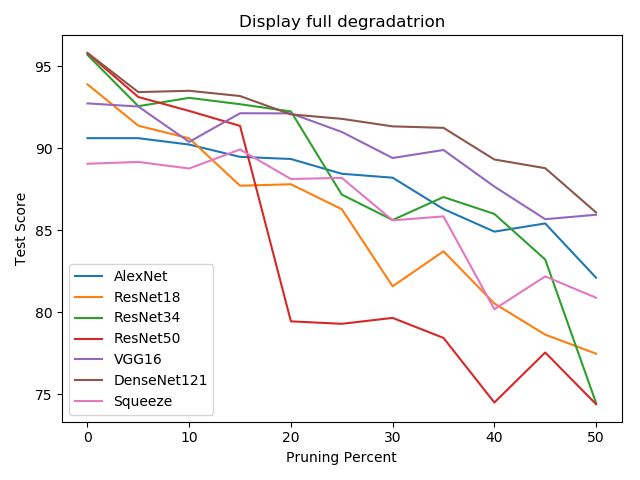
\includegraphics[width=0.30\linewidth]{figures/simple-degrad} & 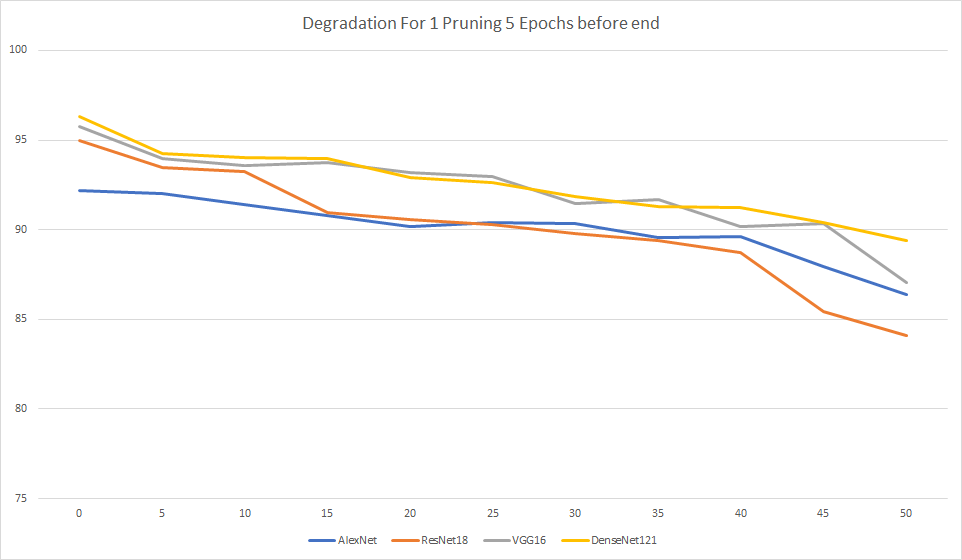
\includegraphics[width=0.30\linewidth]{figures/pruneand5retry} & 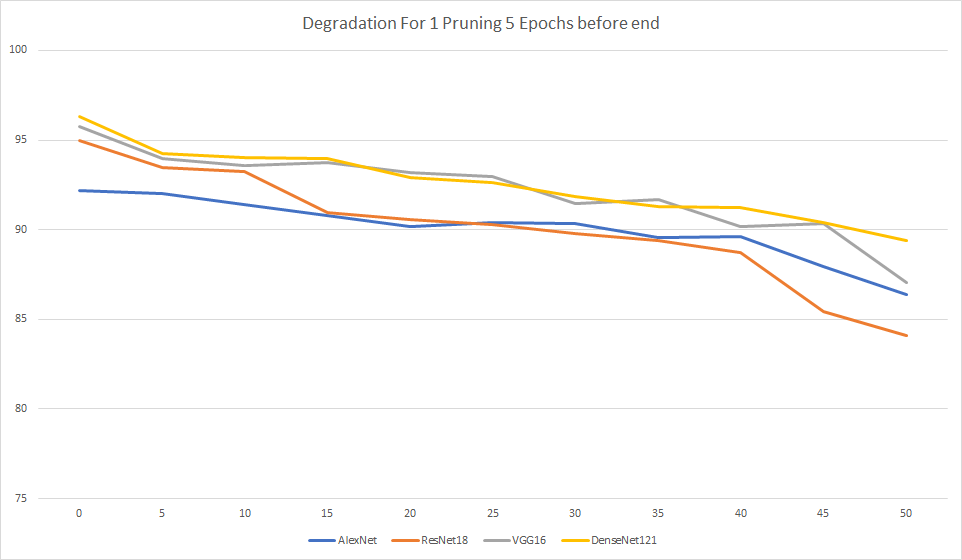
\includegraphics[width=0.30\linewidth]{figures/2pruneand5retry}  \\ 
	\end{tabular}

\begin{tabular}[width=1.00\linewidth]{ccc}
	\multirow{3}{*}{\parbox{0.25\linewidth}
		{The first thing we realize is that if we wait until the end to start our pruning we may expect a greater degradation of our results. Also we see that the result contains some spikes. This seems to indicate that one training after the pruning is not always enough to stabilise the model.}} 
	& 
	\multirow{3}{*}{\parbox{0.25\linewidth}
		{When doing 1 step of pruning once the model start to stabilize will produce consistently higher results. Also the difference between model is a lot less important across the range.}} 
	& 
	\multirow{3}{*}{\parbox{0.25\linewidth}
		{This is a very long line of text}}  \\ 
\end{tabular} 
	


	

\end{center}
}
\end{columns}


\begin{columns}
  \column{.5}
  \block{Observations}
  {
  	\begin{itemize}
   \item Not all convolutional layer can be pruned. Pruning layers before a residual connection is dangerous because both side of the residual connection must have the same side.
  \item When pruning in a convolution layer it is important to propagate to the following layers so the next layers have the right input size. This apply to convolution, linear and batchnorm layers..
  \item It is been seen that algorith leave only one filter on a layer. When this happen it reduce the quality of the results.
  \item When pruning it is important to reset optimizer.
  \end{itemize}
\vspace{0.5cm}
  }

  \column{.5} 
  \block{Conclusion}{
  \vspace{1.0cm}
  \textbf{Discussion:}
    \begin{itemize}
        \item It is a  \colorbold{possible} to support multiple model type using the same module.
        \item The reduction on some model is \colorbold{impressive} and could be run on lower trier hardware.
    \end{itemize}
    
    \textbf{Future Works:}
    \begin{itemize}
        \item  Pruning proved to be a valid form of regulation.
        \item  Would be possible to use different criteria to sort filters.
        \item  Experiments were made on Cifar10. It would be interesting to try on various datasets.
    \end{itemize}
    \vspace{1.6cm}
  }
\end{columns}

\end{document}
